In this section, we demonstrate a typical usage scenario of our tool. Let's say the user is interested in all papers that address the problem of "global illumination". This is one of the fundamental, long-standing problems in computer graphics.

We start by looking at the keywords and clicking on "global" and "illumination". These keywords can be found by either starting the search at the letter "G" and "I", or by using the search textbox. Once these two keywords are clicked on, other related keywords are also highlighted (Figure \ref{fig:global_illumination_selected}).

\begin{figure}[ht]			
    \centering
    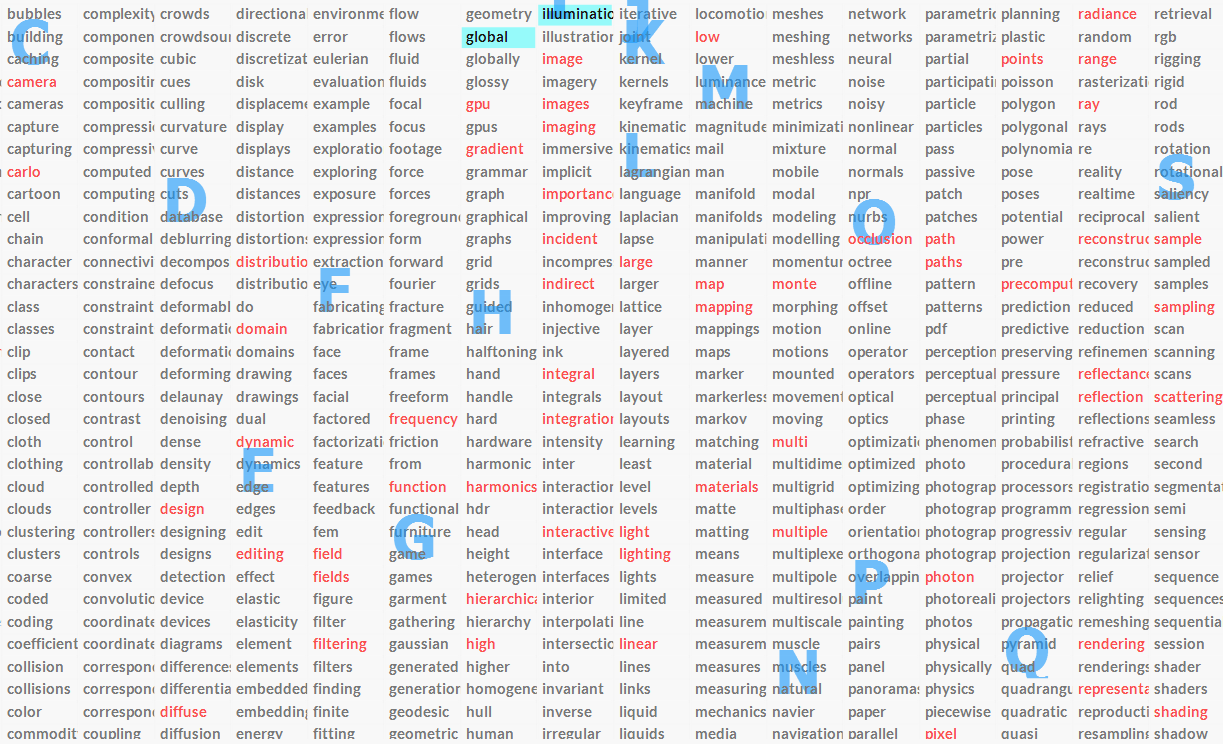
\includegraphics[width=0.7\textwidth]{global_illumination_clicked.png}
    \caption{"global" and "illumination" keywords selected}
    \label{fig:global_illumination_selected}
\end{figure}

In the paper view, papers with both the keywords are highlighted (Figure \ref{fig:global_illumination_papers}).

\begin{figure}[ht]			
    \centering
    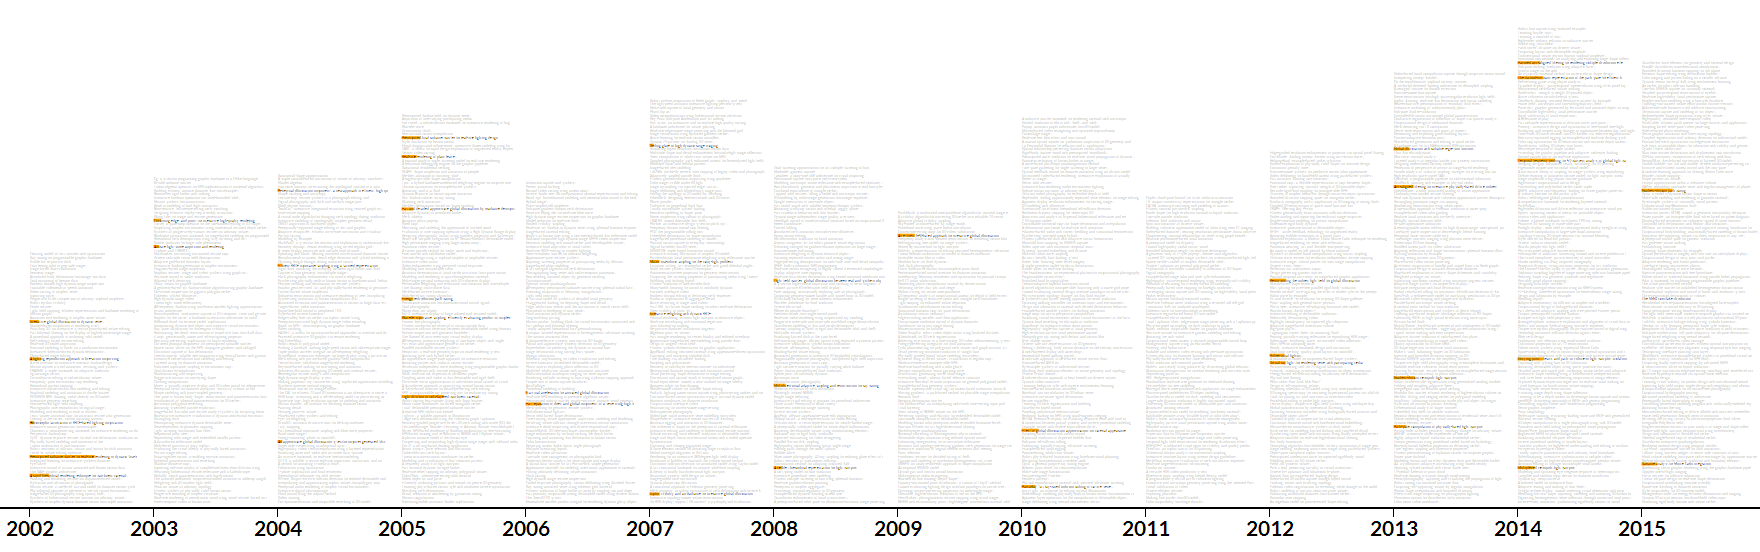
\includegraphics[width=0.7\textwidth]{global_illumination_papers.png}
    \caption{Papers with both keywords: "global" and "illumination" keywords selected}
    \label{fig:global_illumination_papers}
\end{figure}

There are two highlighted papers in 2015, one of them having significantly more citations than the other. Since we are interested in the state-of-the-art research, we click on the one in 2015 with more citations. This paper is called "Gradient domain path tracing" (Figure \ref{fig:gradient_domain_path_tracing_paper_selected}).

\begin{figure}[ht]			
    \centering
    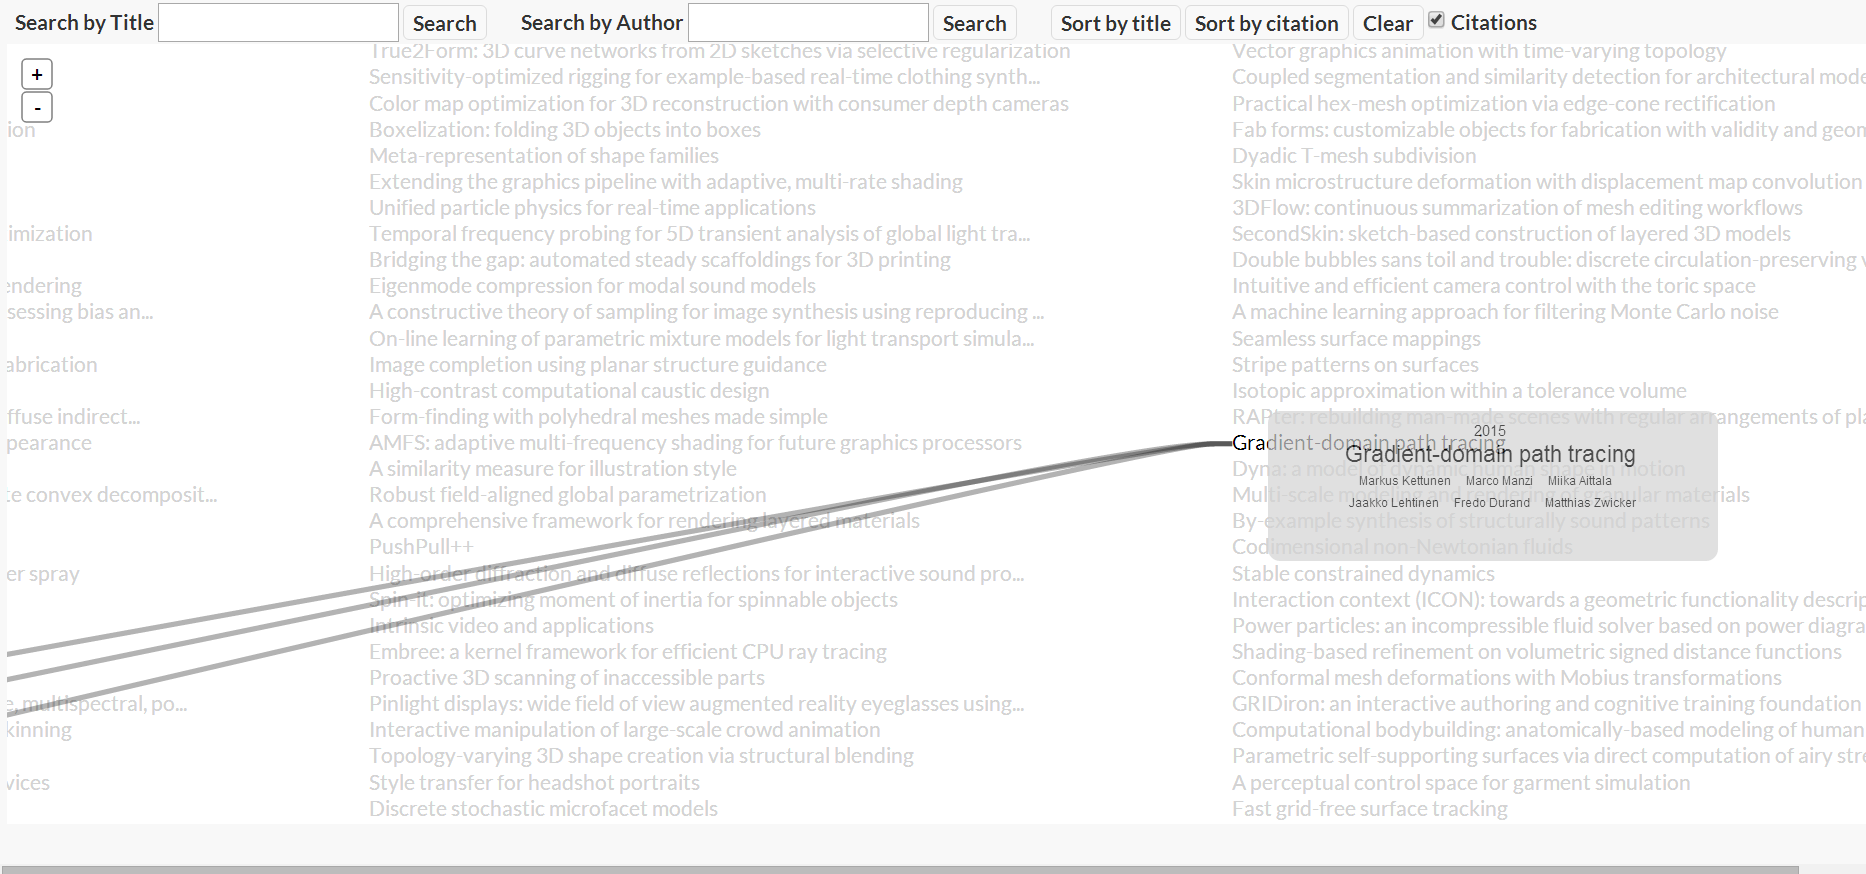
\includegraphics[width=0.7\textwidth]{gradient_domain_path_tracing.png}
    \caption{"Gradient domain path tracing" paper selected}
    \label{fig:gradient_domain_path_tracing_paper_selected}
\end{figure}

In the paper detail view, we can read the selected paper's abstract, as well as see a list of keywords associated with this paper (Figure \ref{fig:gradient_domain_path_tracing_paper_detail}).

\begin{figure}[ht]			
    \centering
    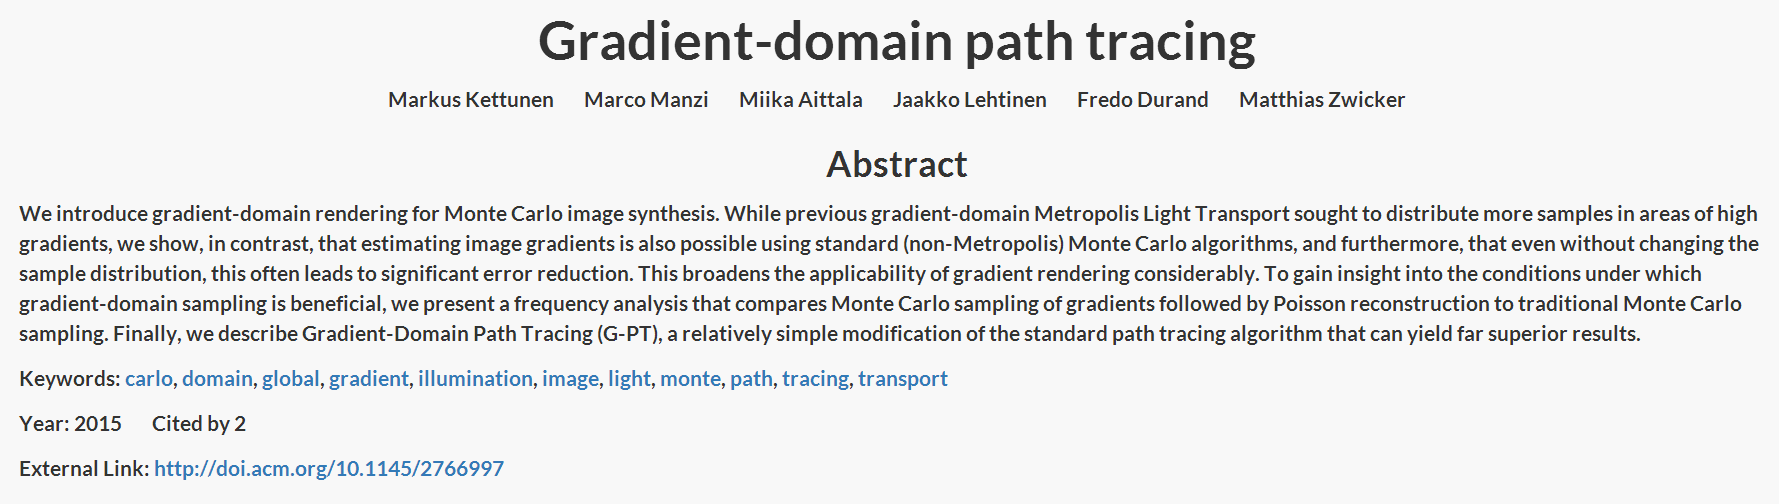
\includegraphics[width=0.7\textwidth]{gradient_domain_path_tracing_detail.png}
    \caption{"Gradient domain path tracing" paper abstract}
    \label{fig:gradient_domain_path_tracing_paper_detail}
\end{figure}

After reading the abstract and having a look at the keywords, we are interested in the keyword "path tracing", which is a technique to achieve global illumination. Clicking on these two words ("path" and "tracing") in the paper detail view bring us to the keyword view where these two keywords are selected (in addition to "global" and "illumination" which were selected before). Going back to the paper view, which now highlights all the papers with these four keywords. Looking at the recent years we notice there are two highlighted papers, one of which is the one that we have already seen (Figure \ref{fig:global_illumination_path_tracing_papers}).

\begin{figure}[ht]			
    \centering
    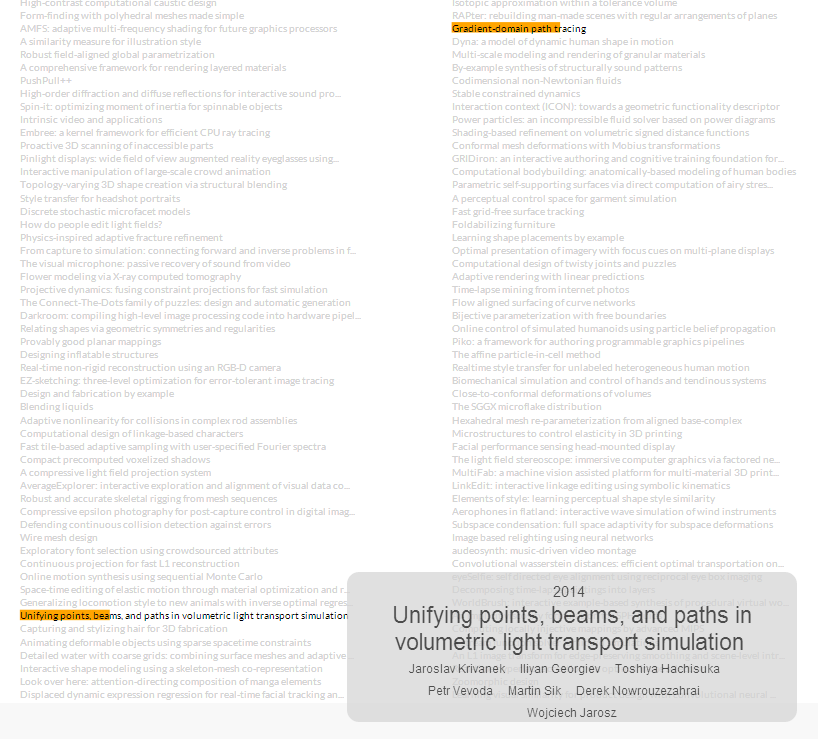
\includegraphics[width=0.7\textwidth]{global_illumination_path_tracing_papers.png}
    \caption{Papers having the four keywords "global", "illumination", "path" and "tracing"}
    \label{fig:global_illumination_path_tracing_papers}
\end{figure}

We click on the the other paper which is titled "Unifying points, beams, and paths in volumetric light transport simulation". After going to the paper detail view to read its abstract, we are interested in this paper and want to find papers that are related to it. We go back to the paper view and see that this paper references another paper in the same year, with a title that seems like it could be of interest to us: "Multiplexed metropolis light transport" (Figure \ref{fig:multiplexed_metropolis_light_transport_referenced}).

\begin{figure}[ht]			
    \centering
    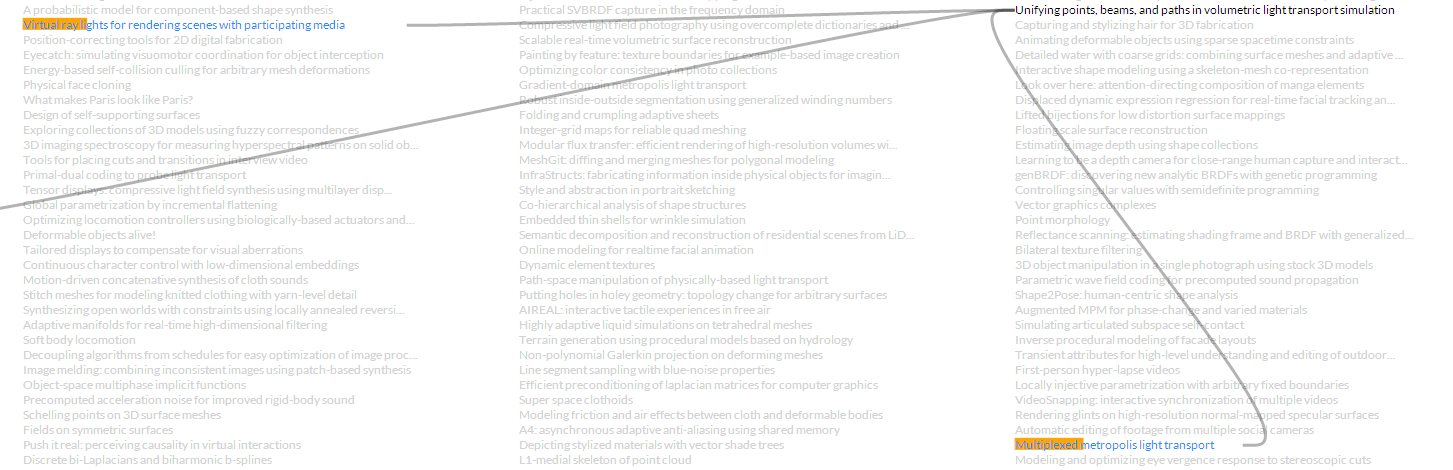
\includegraphics[width=0.7\textwidth]{multiplexed_metropolis_light_trasnport_referenced.png}
    \caption{Papers that our paper of interest references}
    \label{fig:multiplexed_metropolis_light_transport_referenced}
\end{figure}

Clicking on the paper "Multiplexed metropolis light transport", we can read its abstract and furthermore look at its authors. We notice that one of its authors, Carsten Dachsbacher, has written a paper in SIGGRAPH 2007 about a method that addresses the problem of "interactive global illumination" (the paper's title is "Implicit visibility and antiradiance for interactive global illumination") (Figure \ref{fig:carsten_dachsbacher}. We are interested in knowing more about this paper because unlike path tracing, which is a general but very slow solution to the problem of global illumination, this paper seems to propose a method that can compute global illumination at interactive rates.

\begin{figure}[ht]			
    \centering
    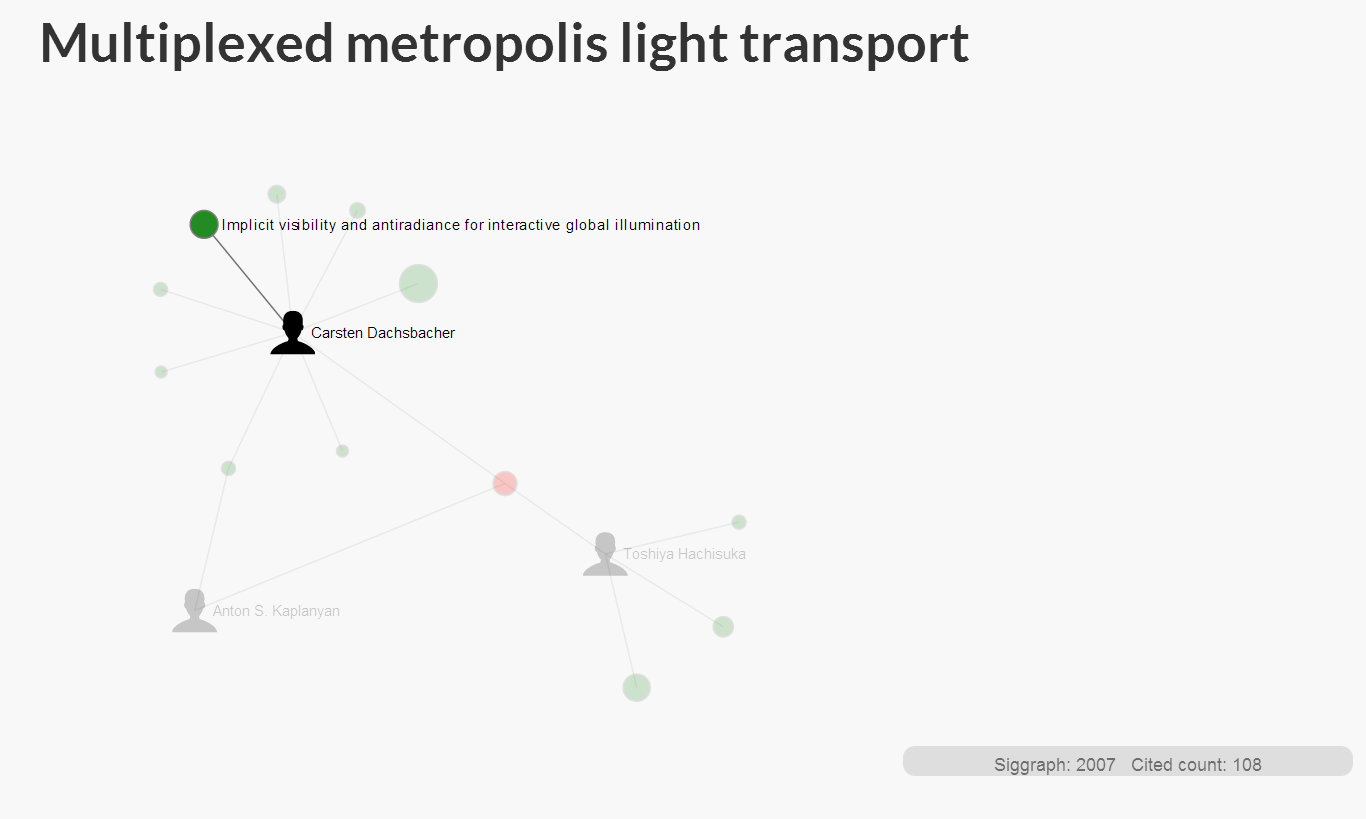
\includegraphics[width=0.7\textwidth]{carsten_dachsbacher.png}
    \caption{Carsten Dachsbacher's SIGGRAPH publications}
    \label{fig:carsten_dachsbacher}
\end{figure}

We then click on the paper "Implicit visibility and antiradiance for interactive global illumination" in the author view to select it. Back to the paper detail view we can read this paper's abstract and look at the list of papers that it references (Figure \ref{fig:antiradiance}). And from this we can continue our exploration of the space of papers that try to solve the global illumination problem in one way or another.

\begin{figure}[ht]			
    \centering
    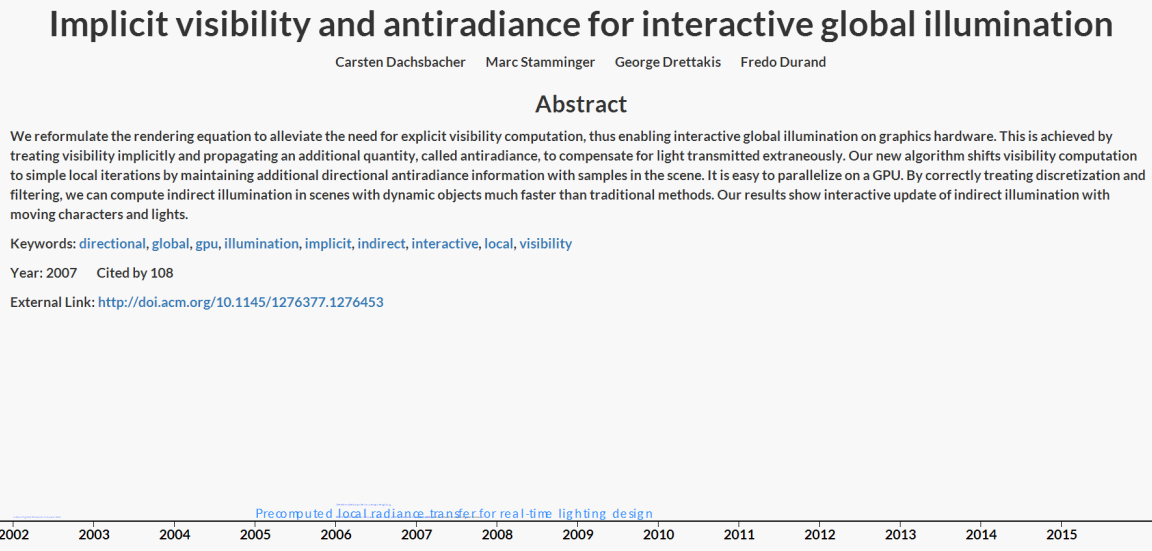
\includegraphics[width=0.7\textwidth]{antiradiance_paper_detail.png}
    \caption{Antiradiance paper details}
    \label{fig:antiradiance}
\end{figure}

\textbf{Conclusion}
We have shown that our tool provides several ways to navigate the space of papers that are related to certain topics of interest. One can use either the reference relationships, the common keyword relationships, or the common author relationships to get to the papers of interest and read their abstract to understand them more. On our way of exploring the data, we also  learn more about the various techniques employed and get an idea about who publish frequently in this topic. All of these can work together to help the user quickly get a high-level understanding of the field of research he or she is interested in.